Die zwei horizontal beweglichen Kolben ($A_2$ und $A_3$) sind mit einem Draht verbunden. Auf dem senkrecht beweglichen Kolben $A_1$ liegt ein Körper der Masse $m$.

\begin{center}
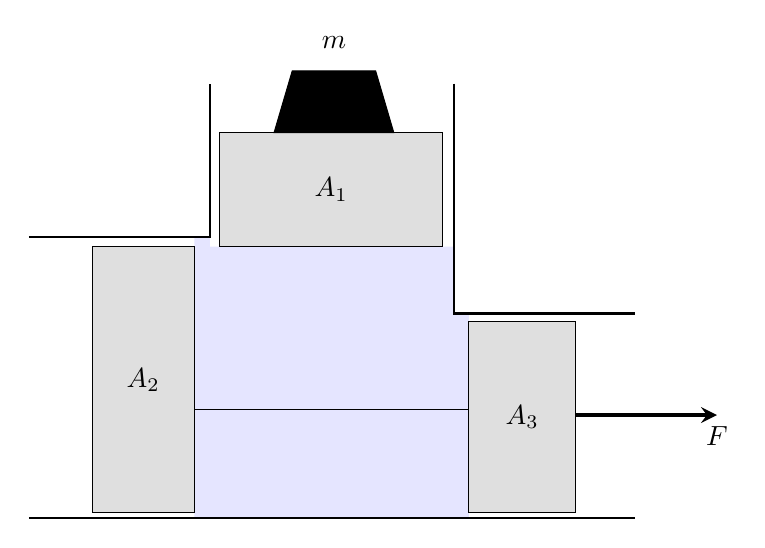
\begin{tikzpicture}[>=stealth, scale=1.15]
 \fill[blue!10] (1.83,0) -- (4.86,0) -- (4.86,2.26) -- (4.70,2.26) -- (4.70,3.0) -- (2.0,3.0) -- (2.0,3.11) -- (1.83,3.11) -- cycle;
 \draw[thick] (0,3.11) -- (2.0,3.11) -- (2.0,4.8);
 \draw[thick] (4.70,4.8) -- (4.70,2.26) -- (6.70,2.26);
 \draw[thick] (0,0) -- (6.70,0);
 \draw[fill=gray!25] (2.11,3.0) rectangle (4.57,4.26) node[pos=0.5] {$A_1$};
 \draw[fill=black] (2.71,4.26) -- (4.03,4.26) -- (3.83,4.94) -- (2.91,4.94) -- cycle;
 \node at (3.37,5.25) {$m$};
 \draw[fill=gray!25] (0.70,0.06) rectangle (1.83,3.0) node[pos=0.5] {$A_2$};
 \draw[fill=gray!25] (4.86,0.06) rectangle (6.04,2.17) node[pos=0.5] {$A_3$};
 \draw (1.83,1.2) -- (4.86,1.2);
 \draw[->, line width=1.5pt] (6.04,1.14) -- (7.6,1.14) node[below] {$F$};
\end{tikzpicture}
\end{center}

\begin{abcliste}
\abc Wie gross ist der Druck zwischen den beiden Kolben?
\abc Wie gross muss die Kraft $F$ sein, damit das System im Gleichgewicht ist?
\end{abcliste}
Zahlenwerte: $A_1 = \AeaO$, $A_2 = \AebO$, $A_3 = \AecO$, $m = \mkoO$
